\documentclass[a4,12pt]{article}

\usepackage[utf8]{inputenc}
\usepackage[spanish]{babel}
\usepackage[margin=1.5cm]{geometry}
\usepackage{graphicx}
\usepackage{color}
\usepackage{import}
\usepackage{float }



\usepackage{hyperref}

\parindent 0em

%\usepackage{times}
\renewcommand{\familydefault}{\sfdefault}

\title{Resolución de problemas a GNU OCTAVE}
\author{Lamya Hafs}
%\date{}

\begin{document}

\maketitle
\bigskip
\bigskip
\bigskip
\begin{figure}[H]
  \centering
    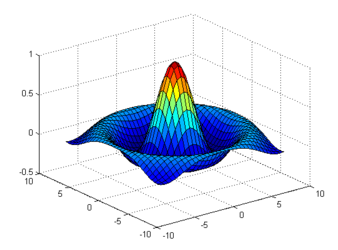
\includegraphics{imagenes/octave}
\end{figure}
\newpage

\maketitle

\begin{abstract}
El documento explica como se ha conseguido resolver problemas mediante el software GNU Octave, se ha elegido dos problemas.\\
- Problema de programacion lineal propuesto en la parte de MatApl "El problema de dieta".\\
- Problema de ordenamiento rápido "Quicksort".\\

\end{abstract}

\tableofcontents
\newpage

\section{El problema de dieta}

\subsection{Discripción del problema}
Se desea añadir a la dieta de ciertos animales de granja cantidades extra de tiamina, fósforo y hierro.\\
Para ello en el mercado existen dos preparados en polvo diferentes: Fosfatón y Ferroforo. Estos
contienen los nutrientes en las cantidades que se indican a continuación. Cada onza de Ferroforo
contiene 0.15 mg de tiamina, 0.75 mg de fósforo y 1.30 mg de hierro. Cada onza de Fosfatón contiene 0.10 mg de tiamina, 1.70 mg de fósforo y 1.10 mg de hierro. Deseamos que cada animal reciba al día, al menos 1.00 mg de tiamina, 7.50 mg de fósforo y 10.00 mg de hierro.\\
El costo de cada onza de Ferroforo es de 0.02 euros y el de Fosfatón es de 5/3 de céntimo de euro poronza. Determinar las cantidades de Ferroforo y Fosfatón que debemos suministrar a cada animal de forma que el costo de este suplemento a la dieta sea mínimo.\\

\subsection{Solución}
En primer lugar expresamos los datos del problema en forma de tabla, lo que nos dará una mejor
perspectiva de los mismos:\\

\begin{center}
\begin{tabular}{|c|c|c|c|c|} \hline
\textbf{Ingredientes}   &  \textbf{Tiamina}  &  \textbf{Fósforo} &  \textbf{Hierro}  &  \textbf{Coste de los igredientes} \\ \hline
Ferroforo  & 0.15 mg/oz  &  0.75 mg/oz & 1.30 mg/oz  &  2 ct/oz  \\  \hline
Fosfatón  & 0.10 mg/oz  &  1.70 mg/oz & 1.10 mg/oz  &  573 ct/oz  \\  \hline
\end{tabular}
\end{center}

\end{document}

